\documentclass[]{article}

\usepackage[numbers]{natbib}
\usepackage{pdflscape}

%opening
\usepackage{float}
\usepackage[hidelinks]{hyperref}
\usepackage{scrextend}
\usepackage[utf8]{inputenc}
\usepackage{graphicx}
\usepackage{listings}
\usepackage{color}
\usepackage{tocloft}
%\renewcommand{\cftpartleader}{\cftdotfill{\cftdotsep}} % for parts
%\renewcommand{\cftchapleader}{\cftdotfill{\cftdotsep}} % for chapters
\renewcommand{\cftsecleader}{\cftdotfill{\cftdotsep}} % for sections, if you really want! (It is default in report and book class (So you may not need it).
\setlength{\parskip}{16pt}

\title{Project Assignment Part II:\@ Simulation of a base scenario }

\author{Jef Jacobs \\ Toon Eeraerts \\ Wout Deleu}
\date{Semester 2}

\begin{document}
\setlength{\parindent}{0pt} \maketitle \tableofcontents \newpage %geen indent bij nieuwe paragraaf

\section{Introduction}
For this assignment, a basic scenario of the `Yard storage assignment problem'
was implemented and simulated. During this report, the basics design choices
will be discussed, as well as the results of the simulation.

The basic technology used is Python. The code is written as dynamic as
possible, using global variables and booleans to variate parameters and the
overall flow of the simulation. It is based on a discrete event simulation,
with the possibility of online simulation.

To refresh the environment in brief, the goal is to simulate a yard, in which
containergroups\footnote{Containers arrive only in group. Containers are (for
	now) not looked at individually. This means they can't be split up, they are
	stored in the same place, they enter and leave the yard at the same time.} come
and go. They can arrive from vessels or from trucks and trains. Each container
needs to be stored on the yard for a specific duration. The goal is to simulate
the storage situations in the yard, as a result of the in and out flow.

\section{Simulation parameters}
The first and maybe most primary parameter to know is the amount of simulations
that needs to be run to get significant results. This can be calculated by the
following formula: \[S = \sqrt{\frac{\sum_{i = 1}^{n}(X_i-\overline{X})^2}{n
			-1}}\] \[\frac{S}{\sqrt{k}} < d\]

The resulting value of the simulation we wanted to take in account, is the
travel distance. So travel distance and average travel distance will be the
factor which we will evaluate the variance on.

S the sample variance, the variance of our results. The number of simulations,
so the value we want to calculate is k. The accepted standard deviation is d.
This is a threshold we want to achieve, and can be chosen in function of the
given results. X represents a system result of the simulation. In our case is
this the average or total travel distance gotten from running the simulation.
When the sample variance based on the k values is within an acceptable range,
the calculation is stopped and the value of k is chosen for the amount of
simulations that needs to be run.

The acceptable deviation differs for the average and total travel distance. For
the average travel distance the deviation chosen is 0.1. This is a low value,
but given the speed of execution and the and magnitude of this value, it was a
achievable. For the total distance the accepted deviation is 1000. If we look
at the magnitude of the total travel distance, we see it surpasses a million. A
deviation of a thousands seems in that case reasonable. The total distance
travelled is a much larger value than the average distance, because of this the
accepted deviation is larger.

\begin{figure}[!tbp]
	\centering
	\begin{minipage}[b]{0.44\textwidth}
		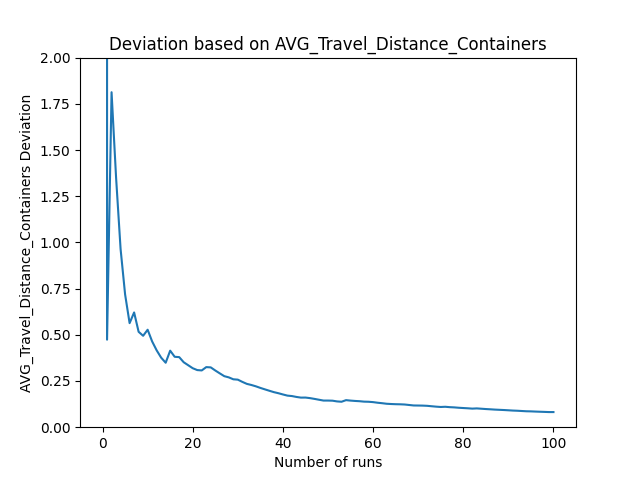
\includegraphics[width=\textwidth]{Afbeeldingen/deviation_avg_distance.png}
		\caption{Deviation average travel distance of the containers}\label{fig:deviation}
	\end{minipage}
	\hfill
	\begin{minipage}[b]{0.44\textwidth}
		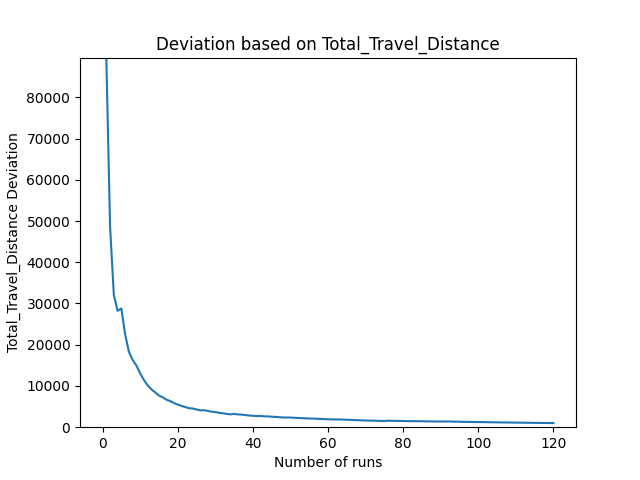
\includegraphics[width=\textwidth]{Afbeeldingen/deviation_total_distance.png}
		\caption{Deviation total travel distance of the containers}
	\end{minipage}
\end{figure}

The deviation of the average distance travelled is 0.082 after 100 runs. The
deviation of the total distance travelled is 997.08 after 120 runs. The
evolution of the deviation for both features is shown in figure~\ref{fig:
	deviation}. In the graph of the average distance, the beginning has more
fluctuations than the graph of the total travel distance. This is because the
deviation is far smaller than the total distance deviation. From this
information we can conclude that at least 120 simulations must be done to get
consistent results.

\subsection{Generation of parameters}
In order to emulate the basic behavior of the yard, there needs to be a stream
of containergroups, with their own properties. To perform an online simulation,
this stream needs to be generated on the fly. In the prior assignment, a study
was held to figure out distributions, which will be used to generate the
necessary information regarding the containergroups. This is necessary to
generate the input to feed the simulation.

The generation of these groups happens at random times, which are calculated
using the arrival time of the previous group, and a random inter arrival time.
This interval time is being generated using an exponential function based upon
the input data analysis of Nick De Bruyckere, Enrique Miron and Dries Van de
Velde (Figure \ref{fig: inter arrival time analysis}).
\begin{figure}[!tbp]
	\centering
	\begin{minipage}[b]{0.40\textwidth}
		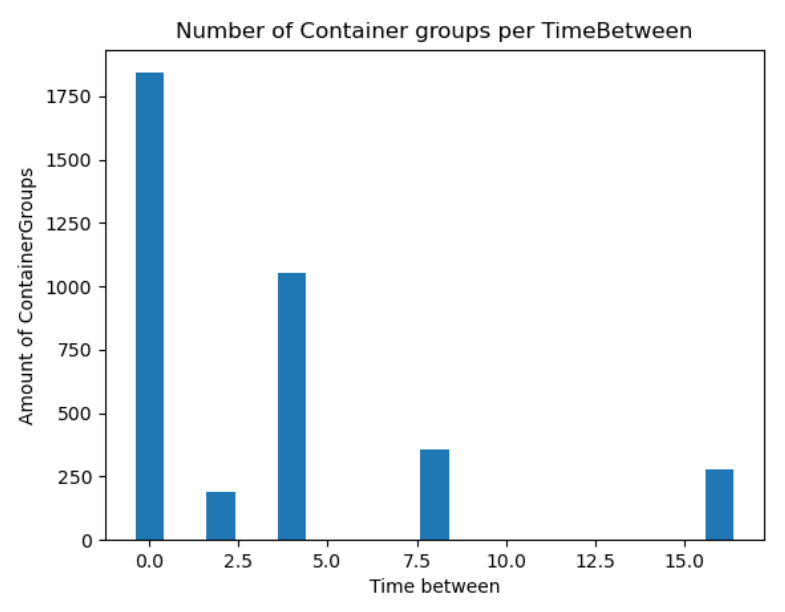
\includegraphics[width=\textwidth]{Afbeeldingen/inter_arrival_times_hist.png}
		\caption{Inter arrival time in prior analysis}
		\label{fig:inter arrival time analysis}
	\end{minipage}
	\hfill
	\begin{minipage}[b]{0.44\textwidth}
		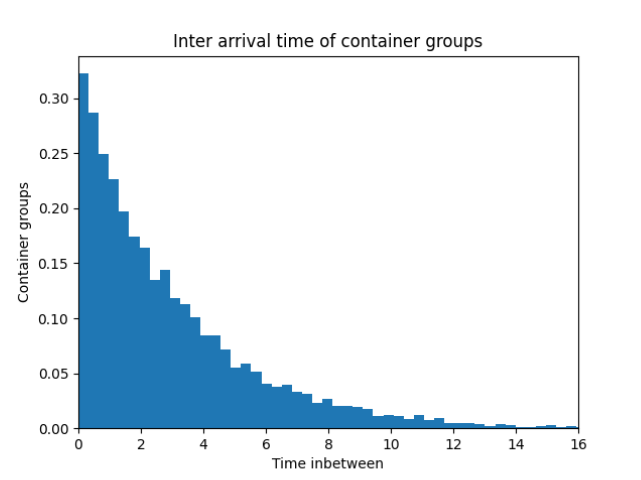
\includegraphics[width=\textwidth]{Afbeeldingen/inter_arrival_time_sample.png}
		\caption{Inter arrival time sample distribution used in the simulation}
	\end{minipage}
\end{figure}

When the arrival time of a batch of containers is determined, some properties
of that container group needs to be generated. The properties are:
\begin{itemize}
	\item The type of containers
	\item The number of containers in the group
	\item The service time needed
	\item The arrival position of the group
	\item The departure position of the group
	\item The flow type (which can be import or export)
\end{itemize}

The type of containers is also based upon the input analysis of Nick De
Bruyckere, Enrique Miron and Dries Van de Velde represented in Figure~\ref{fig:
	container type analysis}. Normal containers and reefer container occur
respectively 69\% and 31\% of the times.
\begin{figure}
	\centering
	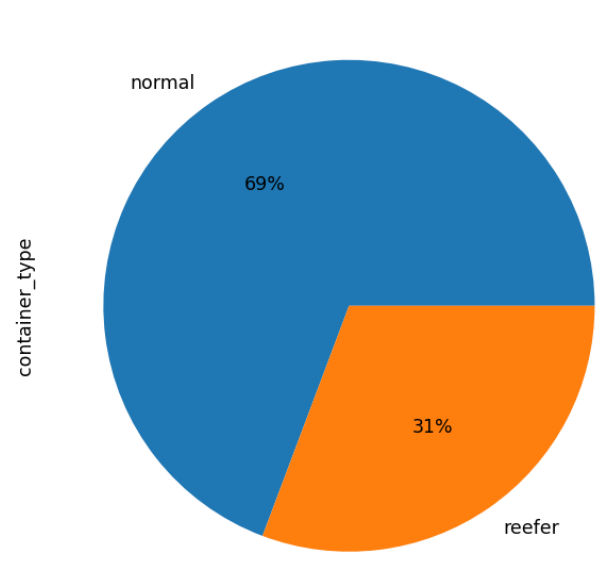
\includegraphics[width=0.5\textwidth]{Afbeeldingen/container_type.png}
	\caption{Container type analysis}
	\label{fig:container type analysis}
\end{figure}

Each group has a certain amount of containers in them. This is chosen based
upon our own analysis of the input data. The distribution is represented by a
steep exponential distribution which is never lower than 1. (Figure: \ref{fig:
	container group size sample})
\begin{figure}[!tbp]
	\centering
	\begin{minipage}[b]{0.45\textwidth}
		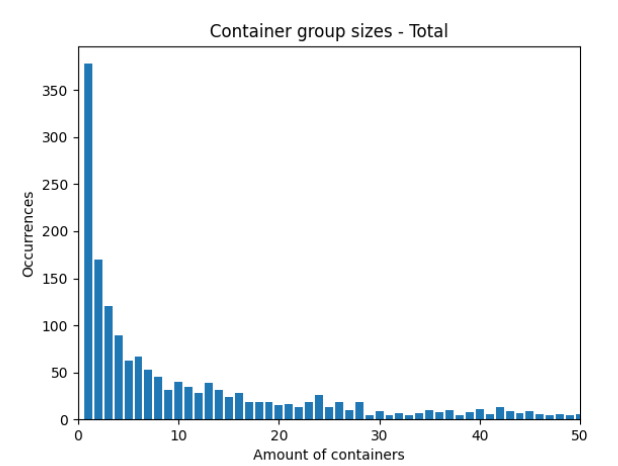
\includegraphics[width=\textwidth]{Afbeeldingen/container_group_sizes.png}
		\caption{container group size analysis}
	\end{minipage}
	\hfill
	\begin{minipage}[b]{0.44\textwidth}
		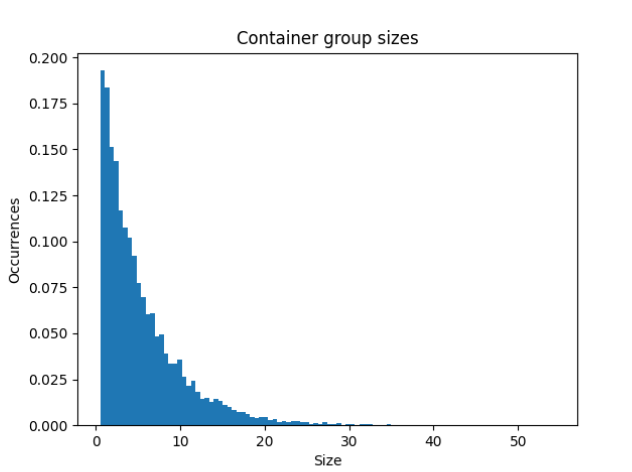
\includegraphics[width=\textwidth]{Afbeeldingen/container_group_size_sample.png}
		\caption{Container group size sample distribution}
		\label{fig:container group size sample}
	\end{minipage}
\end{figure}

Each instance has a service time, which is the time containers need to stay in
the yard before further actions are taken. This factor is directly dependent on
the flow type. If it is import or export, the service time is by default 48
hours. But if it is stated as a transhipment (which is technically a subtype of
export), it can vary between 0 and 166 hours. This is based upon our own
analysis of the input data which shows a somewhat uniform distribution between
0 and 166 hours (Figure~\ref{fig: service time analysis}). For this reason, the
service time sample always takes a random number between these two values.
\begin{figure}
	\centering
	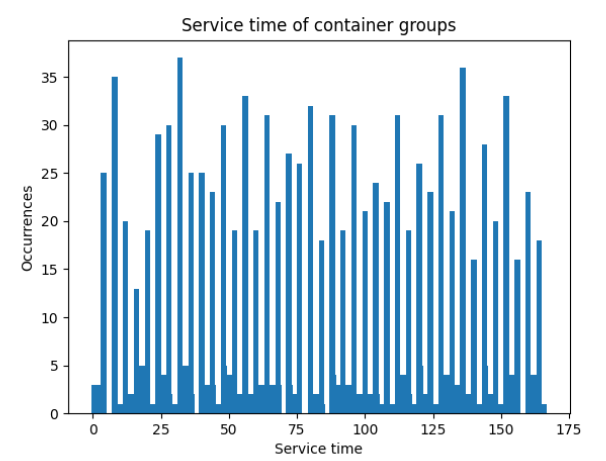
\includegraphics[width=0.5\textwidth]{Afbeeldingen/service time analysis.png}
	\caption{Service time analysis}
	\label{fig: service time analysis}
\end{figure}

The arrival and departure position of vessels and trucks is randomly selected
out of the available locations.

\subsection{Resulting values}
Each simulation run will store different characteristics which will be used to
evaluate the performance of the simulation. The most important characteristics
are: \begin{itemize}
	\item Amount of rejected containers and container groups (total and for each type
	      individually)
	\item The total and average travel distance
	\item Per YardBlock:
	      \begin{itemize}
		      \item The maximal occupancy at any given time
		      \item The maximal occupancy per day (\textbf{= average occupancy per day})
	      \end{itemize}
	\item Average daily occupancy over all containers: The average occupancy per day over
	      all the YardBlocks \[\forall i \in days: \frac{\sum_{(x \in YardBlocks)}
			      \overline{Occupancy_{i,x}}}{\#YardBlocks}\]
\end{itemize}

After seeing the first results, it was clear that with 159 yardblocks in total,
it is not the most useful thing to list the individual occupancy for every
block, and include this in this rather short report. But to give an idea of
this data, some basic statistics are given over the data: \begin{itemize}
	\item The amount of YardBlocks which are close to being full (90\% average
	      occupancy\footnote{\label{margin} Because the simulation is run many times,
		      averages of 100\% for example are extremely hard to reach, thats why a small
		      margin of 10\% has been taken into account.})
	\item The amount of YardBlocks which are never used (5\% average
	      occupancy\footref{margin})
\end{itemize}

\section{Results}

\subsection{Basic scenario}
The basic scenario that is discussed in this report describes a decision rule
which stores every containergroup that arrives, if there is space in the yard.
This will be referred to as \textit{FIFO (First In First Out)}. This apply's to
arrival of containers, and wether or not they are stored in the yard. FIFO says
that the first container that arrives, has a priority over the ones which
arrive after the first one. If there is no space for an arriving
containergroup, it will be rejected. While the next containergroup arrives, the
check for space will happen again, and so on.

Two different approaches to block assignments are implemented. The block
assignment rule has affect on which block is chosen to store a containergroup.
The two different situations studied here are \textit{arrival based} and
\textit{departure based}. Arrival based and departure based are both based on
the minimal distance between 2 points. The yard block chosen is the closest
block to the arrival point, in case of arrival based, or closest to the
departure point, in case of departure based.

The 2 different approaches give somewhat similar results. The main difference
is in the travel distance. This is significantly higher with departure based
approach. This could be explained by the fact that groups leave the yard on
more similar positions, than they arrive, which could lead to yardblocks
getting full, and so containers being stored somewhat further from their
optimal point. This is a rather unlikely scenario, because individual blocks
are (almost) never even close to full. It is consequently unlikely that
containergroups would be stored somewhere else than it's optimal position.
Another more likely explanation is that the temporary storage point found for
containers on the yard in the departure based implementation is further from
the optimal route than when searching for the closest block to the arrival
point. This can maybe a vague description, but Figure~\ref{fig:closest} could
clarify this. Point \textbf{A} could be an arrival point, point \textbf{B} a
departure point.~\textbf{C1} is the yardblock closest to the arrival point, and
\textbf{C2} to the departure point. The shortest path from A to B is the
straight line. We can see that C2 is further from the optimal path than C1. In
other words, there are more blocks available close to arrivals (and closer to
the arrival points) than to departure points. Trucks have in the current
implementation only four possible location. This is approximately ten times
less than the amount of berthlocations.
\begin{figure}
	\centering
	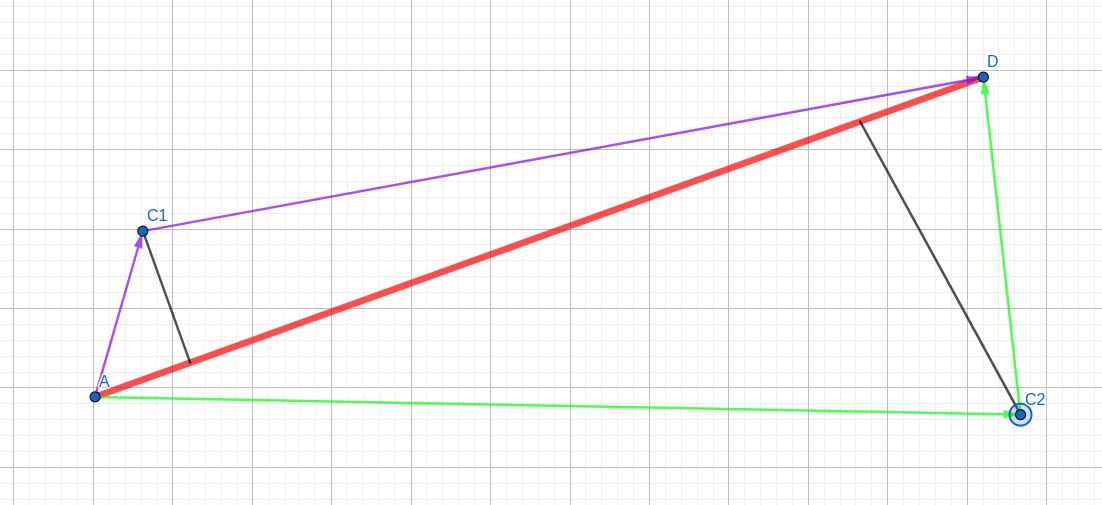
\includegraphics[width=0.7\linewidth]{Afbeeldingen/distances.png}
	\caption{Closest block to arrival and departure point}\label{fig:closest}
\end{figure}

The fact that there are no containers rejected, and the fact that the occupancy
is so low, is noteworthy. This implies that the yard is too big, and the stream
of containers is to little to stress the simulation even in the slightest way.
This could imply that the stream of containers is to light for this yard.
\begin{table}[h]
	\centering
	\begin{tabular}{|c|c|}
		\hline
		Containers Rejected                         & 0.0        \\ \hline
		CG Rejected                                 & 0.0        \\ \hline
		Normal Rejected                             & 0.0        \\ \hline
		Reefer Rejected                             & 0.0        \\ \hline
		Total Travel Distance                       & 6051683.63 \\ \hline
		AVG Travel Distance Containers              & 380.31     \\ \hline
		AVG daily total Occupancy                   & 0.0366     \\ \hline
		Portion of YB never used                    & 0.7799     \\ \hline
		Portion of YB close to full (at some point) & 0          \\ \hline
		Portion of YB close to full (average)       & 0          \\ \hline
	\end{tabular}
	\caption{FIFO arrival based statistics}
\end{table}
\begin{table}[h]
	\centering
	\begin{tabular}{|c|c|}
		\hline
		Containers Rejected                         & 0.0        \\ \hline
		CG Rejected                                 & 0.0        \\ \hline
		Normal Rejected                             & 0.0        \\ \hline
		Reefer Rejected                             & 0.0        \\ \hline
		Total Travel Distance                       & 7468862.53 \\ \hline
		AVG Travel Distance Containers              & 468.10     \\ \hline
		AVG daily total Occupancy                   & 0.05272    \\ \hline
		Portion of YB never used                    & 0.7799     \\ \hline
		Portion of YB close to full (at some point) & 0          \\ \hline
		Portion of YB close to full (average)       & 0          \\ \hline
	\end{tabular}
	\caption{FIFO departure based statistics}
\end{table}

\subsection{Stressing the system}
The results show that the majority of the yard is not occupied with the normal
distribution values. In order to get more relevant results, the decision was
made to tune parameters, regardless of the samples. The parameters were tuned
in order to get more containers into the yard, to see how it would react to a
more intense input.

A first option could be to decrease the inter-arrivaltimes, so that
containergroups arrive faster. To increase the yard occupancy we can also
increase the size of the containergroups and increase the service time.
Increasing the size of the containergroups has limitations, this is due to the
requirement that containergroups need to be stored in a single yardblock.
Beyond a threshold, increasing the size of the containergroups will result into
a lot of rejected containers without increasing the occupancy. Removing the
constraint that containers from a container group can only be stored in a
single yardblock would make larger containergroups possible.

Table~\ref{tab: Container rejection analysis} shows the impact of changing
parameters on the rejection of the containers. Table~\ref{tab: yard occupation
	analysis} shows the occupation changes when parameters are changed. When the
containtergroups arrive up to four times faster than usual, no containers get
rejected. Changing the inter-arrivaltime has some impact on the yard occupancy,
however the yard is still quite empty. Decreasing this parameter further is not
efficient due to the impact it has on the simulation time.

To increase the yard occupation the sizes of the containergroups can be upped.
When the containergroup size is increased to five times the normal size, reefer
containers start to get rejected. This is because the largest yardblock for
reefer containers is 171, which is much smaller than the largest normal yard
block which has the size of 836. This is not in proportion to the $31/69$
distribution when generating containers.

The occupancy level of the yard does increase when more containers arrive, but
the yard is still quite empty at five times the containergroup size, with a max
of 8\% occupation.

The service time can be increased to 50 times without having to reject
containergroups. The yard is still relatively empty when increasing the service
time 50 times with a max occupation of 6\%.

In an effort to really stress the yard the three parameters are changed in a
single simulation. The size of the containergroups are increased with two, to
limit the rejections due to the restriction on storing the containergroup into
a single yardblock. When increasing the service time with a factor of 50,
doubling the containers in a group and receiving containers at four times the
usual speed the yard comes closer to getting full. With a max of 48\% and an
average of 15\%. Still 37\% of the yardblocks are never used. Increasing these
parameters has mostly impact on the reefer containers. These containers reach
the limit much faster than the normal containers with 1109 reefer
containergroups rejected and 0 normal containergroups rejected. From this we
can conclude that the reefers are more susceptible to parameter changes than
the normal containers.

\begin{table}[h]
	\centering
	\begin{tabular}{|l|l|l|l|}
		\hline
		Changed parameters                                                                             & CG Rejected & Normal Rejected & Reefer Rejected \\ \hline
		0.5 * interarrival time                                                                        & 0           & 0               & 0               \\ \hline
		0.25 * interarrival time                                                                       & 0           & 0               & 0               \\ \hline
		2 * containers                                                                                 & 0           & 0               & 0               \\ \hline
		5 * containers                                                                                 & 1.03        & 0               & 202.79          \\ \hline
		2 * service time                                                                               & 0           & 0               & 0               \\ \hline
		5 * service time                                                                               & 0           & 0               & 0               \\ \hline
		10 * service time                                                                              & 0           & 0               & 0               \\ \hline
		20 * service time                                                                              & 0           & 0               & 0               \\ \hline
		50 * service time                                                                              & 0           & 0               & 0               \\ \hline
		\begin{tabular}[c]{@{}l@{}}50 * service time \\ 2 * containers\\ 0.25 * interarrival time\end{tabular} & 1109.8      & 0               & 21148.5         \\ \hline
	\end{tabular}
	\caption{Container rejection analysis}\label{tab: Container rejection analysis}
\end{table}

\begin{table}[h]
	\centering
	\begin{tabular}{|l|l|l|l|l|}
		\hline
		Changed parameters                                                                             & AVG Occupancy & YB never used & YB close to full AVG & YB close full Max \\ \hline
		0.5 * interarrival time                                                                        & 0.015         & 0.735         & 0.006                & 0.0125            \\ \hline
		0.25 * interarrival time                                                                       & 0.0243        & 0.729         & 0.006                & 0.018             \\ \hline
		2 * containers                                                                                 & 0.016         & 0.729         & 0.006                & 0.0125            \\ \hline
		5 * containers                                                                                 & 0.03          & 0.622         & 0.006                & 0.0817            \\ \hline
		2 * service time                                                                               & 0.0133        & 0.748         & 0.006                & 0.006             \\ \hline
		5 * service time                                                                               & 0.0139        & 0.735         & 0.006                & 0.0125            \\ \hline
		10 * service time                                                                              & 0.02974       & 0.723         & 0.006                & 0.0125            \\ \hline
		20 * service time                                                                              & 0.0481        & 0.71          & 0.006                & 0.0314            \\ \hline
		50 * service time                                                                              & 0.0856        & 0.6729        & 0.0125               & 0.061             \\ \hline
		\begin{tabular}[c]{@{}l@{}}50 * service time \\ 2 * containers\\ 0.25 * interarrival time\end{tabular} & 0.409         & 0.37          & 0.1572               & 0.48              \\ \hline
	\end{tabular}
	\caption{yard occupation analysis}\label{tab: yard occupation analysis}
\end{table}

\section{Conclusion}
We can conclude that using sampling based on the original is not sufficient to
really stress the yard. The yard is to big, or the flow is to light. A second
point is the fact that there could be a real impact of the fact that there are
only four arrivalpoints for trucks, which could really impact the travel time.
The arrival based implementation is the better choice.

While stressing the system, it can be said that the generation progress of
reefers relative to the normal containers is not in proportion to the storage
capacity of them. The bottleneck are the reefer containers. A last conclusion
is the same as the first one, the yard is to big or the flow is to light. And
while tweaking parameters, it is clear it is far to light. We need to push the
system in rather extreme ways to get the yard to fill up.

\end{document}